% Options for packages loaded elsewhere
\PassOptionsToPackage{unicode}{hyperref}
\PassOptionsToPackage{hyphens}{url}
%
\documentclass[
]{article}
\usepackage{lmodern}
\usepackage{amssymb,amsmath}
\usepackage{ifxetex,ifluatex}
\ifnum 0\ifxetex 1\fi\ifluatex 1\fi=0 % if pdftex
  \usepackage[T1]{fontenc}
  \usepackage[utf8]{inputenc}
  \usepackage{textcomp} % provide euro and other symbols
\else % if luatex or xetex
  \usepackage{unicode-math}
  \defaultfontfeatures{Scale=MatchLowercase}
  \defaultfontfeatures[\rmfamily]{Ligatures=TeX,Scale=1}
\fi
% Use upquote if available, for straight quotes in verbatim environments
\IfFileExists{upquote.sty}{\usepackage{upquote}}{}
\IfFileExists{microtype.sty}{% use microtype if available
  \usepackage[]{microtype}
  \UseMicrotypeSet[protrusion]{basicmath} % disable protrusion for tt fonts
}{}
\makeatletter
\@ifundefined{KOMAClassName}{% if non-KOMA class
  \IfFileExists{parskip.sty}{%
    \usepackage{parskip}
  }{% else
    \setlength{\parindent}{0pt}
    \setlength{\parskip}{6pt plus 2pt minus 1pt}}
}{% if KOMA class
  \KOMAoptions{parskip=half}}
\makeatother
\usepackage{xcolor}
\IfFileExists{xurl.sty}{\usepackage{xurl}}{} % add URL line breaks if available
\IfFileExists{bookmark.sty}{\usepackage{bookmark}}{\usepackage{hyperref}}
\hypersetup{
  pdftitle={Child survival for mothers: mortality change and related measures},
  pdfauthor={Ivan Williams and Diego Alburez-Gutierrez},
  hidelinks,
  pdfcreator={LaTeX via pandoc}}
\urlstyle{same} % disable monospaced font for URLs
\usepackage[margin=1in]{geometry}
\usepackage{graphicx}
\makeatletter
\def\maxwidth{\ifdim\Gin@nat@width>\linewidth\linewidth\else\Gin@nat@width\fi}
\def\maxheight{\ifdim\Gin@nat@height>\textheight\textheight\else\Gin@nat@height\fi}
\makeatother
% Scale images if necessary, so that they will not overflow the page
% margins by default, and it is still possible to overwrite the defaults
% using explicit options in \includegraphics[width, height, ...]{}
\setkeys{Gin}{width=\maxwidth,height=\maxheight,keepaspectratio}
% Set default figure placement to htbp
\makeatletter
\def\fps@figure{htbp}
\makeatother
\setlength{\emergencystretch}{3em} % prevent overfull lines
\providecommand{\tightlist}{%
  \setlength{\itemsep}{0pt}\setlength{\parskip}{0pt}}
\setcounter{secnumdepth}{-\maxdimen} % remove section numbering
\newlength{\cslhangindent}
\setlength{\cslhangindent}{1.5em}
\newenvironment{cslreferences}%
  {\setlength{\parindent}{0pt}%
  \everypar{\setlength{\hangindent}{\cslhangindent}}\ignorespaces}%
  {\par}

\title{Child survival for mothers: mortality change and related
measures}
\author{Ivan Williams and Diego Alburez-Gutierrez}
\date{07 August 2019}

\begin{document}
\maketitle

\hypertarget{introduction}{%
\subsection{Introduction}\label{introduction}}

Kin count estimation has a long and distinguished pedigree in
mathematical demography, starting with the work of Lotka (1931) on
modelling orphanhood in theoretical populations across demographic
regimes. To the best of our knowledge, Brass (1953) first proposed a
formula to represent child survival over age. The notion of estimating
the expected number of living daughters in a stable population was
generalized by Goodman, Keyfitz, and Pullum (1974) for other kin
relations (granddaughters, cousins, etc.). The ``counting method''
approach was further popularized in Keyfitz and Caswell (2005).
Bongaarts (1987) used a similar approach to estimate descendants in his
`Family Status Model'.

The question of child survival, particularly the survival of daughters
for mothers, sits at the very center of demographic theory. This is
evidenced by the omnipresence of the `net reproductive rate' in accounts
of human and non-human populations. Historical demographers draw
liberally on assumptions about kin availability and individual's
exposure to offspring mortality to explain fertility decisions,
especially around the demographic transition. These assumptions are
often untested given the data sparsity (Livi Bacci 1997; Volk and
Atkinson 2013). Economic theories of fertility that consider children as
`investment' for old-age support also rely on notions of child survival
(Preston and others 1978).

Child survival - and it's counterpart, child death - gain new
significance in the wake of the fertility transition. Depressed
fertility means that fewer children are tasked with providing key
emotional, social, and financial transfers to aging parents for ever
increasing periods of time. With increasing periods of generational
overlap, individuals find themselves `sandwiched' between aging parents
and young children requiring their simultaneous attention and care
(Daatland, Veenstra, and Lima 2010). In the context of global population
aging, elderly parents without access to formal social security and
pension systems are particularly reliant on these transfers to make ends
meet (Smith-Greenaway and Trinitapoli 2020).\\
Losing an only child may become a more common experience in the context
of global fertility decline, something particularly worrying for parents
suddenly rendered childless. Given the known psychological, health, and
social consequences of child loss for bereaved parents and families
(Hendrickson 2009; Lee et al. 2014), it is surprising that the
demographic processes that shape parental bereavement remain very poorly
understood. Recent development have underscored the need to understand
how sudden changes in mortality affect the availability of kin. In the
context of the global pandemic caused by the Covid-19 disease, elderly
people depend on support provided by their relatives, especially during
periods of lockdown and in the absence of governmental support
mechanisms. Elderly parents may be at a higher risk of losing the key
support provided by their adult children given the known age-gradient in
the Covid-19 case fatality rate. How do changes in mortality affect the
availability of offspring over age from the point of view of a
prospective mother? How can we characterize the timing of offspring
mortality as experienced by a mother from a formal demographic
perspective? How this would work in an heterogeneity population? In the
remainder of the paper, we aim to formalize the relationship
population-level changes in mortality rates and perceived change in the
lived experience of child death from the perspective of a mother. Our
approach is key for understanding the impact of age-specific excess
mortality on the resilience or otherwise of kinship networks for the
vulnerable elderly population. We consider the case when these changes
are additive, mutliplicative, and when they are not evenly distributed
across age. In this paper, we uncover formal relationships to answer
these questions and provide numerical applications using data from
countries in Latin America during the second half of the twentieth
century. See the \protect\hyperlink{Data}{data section} in the
\protect\hyperlink{Applications}{Applications} section for more details
on the source, calculation procedures and main results. We used period
measures, in an stable context, so the objetive is give moment measures.
A more sophisticated model using the appropriate age-specific cohort
rates in the subscripts has been proposed by Alburez-Gutierrez, Kolk,
and Zagheni (2019).

\hypertarget{relationship-proof}{%
\subsection{Relationship \& Proof}\label{relationship-proof}}

\hypertarget{child-survival}{%
\subsubsection{Child Survival}\label{child-survival}}

Let \(CS_a\) be the expected number of surviving children to a
mother\footnote{We use woman and mother interchangeably in this paper,
  assuming that all women are exposed to the same fertility rates.}
alive at aged \(a\) in a female stable population with fertility rates
\(m_{x}\), mortality hazard \(\mu_{x}\) and survival function
\(l_x=e^{-\int_{0}^{x}{\mu_t}\,dt}\) (with unit radix \(l_0=1\)), as
proposed by Goodman, Keyfitz, and Pullum (1974):

\[
\begin{aligned}
CS_a = \int_{0}^a{m_{x}l_{a-x}dx}
\end{aligned}
\]

\hypertarget{an-approximation}{%
\subsubsection{An approximation}\label{an-approximation}}

As an initial step, we seek an intuitive understanding of the effect of
changing mortality on child survival. Building on work by Keyfitz and
Caswell (2005) for the probability of a living mother, we show which
features of the child survival function explain the expected number of
children. For this we use an approximate of \(l_x\) using Taylor´s
theorem until second order around the mean age of childbearing
\(\kappa\) for all \(a>=\alpha\):

\[CS_a \approx l_{a-\kappa} \int_{\alpha}^a{m_{x}dx}+(l_{a-\kappa})^{'}\int_{0}^a{(x-\kappa)m_{x}dx}+
(l_{a-\kappa})^{''}\int_{0}^a{\frac{(x-\kappa)^2}{2} m_{x}dx}\\
  \approx F_a l_{a-\kappa} + \frac{\sigma^2}{2}F_a (l_{a-\kappa})^{''}\\
  \approx F_a \, l_{a-\kappa}[1+\frac{\sigma^2}{2}\frac{(l_{a-\kappa})^{''}}{l_{a-\kappa}}]\]

where the fertility pattern by age is concentrated around \(\kappa\) and
the accumulated fertility (or gross reproduction rate in our same-sex
model) is \(F_a = \int_{\alpha}^a{m_{x}dx}\). The second Taylor´s term
is null because \(\int_{\alpha}^a{x \, m_{x}dx} = \kappa \, F_a\).

We find that, seen from the perspective of a mother, child survival
mainly depends on the cummulative fertility function\footnote{Note that
  this runs contrary to the findings of Keyfitz and Caswell (2005), who
  found that levels of fertility did not affect the probability of
  having living ancestors.} and the mean age at childbearing \(\kappa\)
acts through the factor \(l_{a-\kappa}\). The dispersion of of fertility
\(\sigma^2\) is negatively proportional to child survival. All else
constant, a higher dispersion of fertility \(\sigma^2\) is associated
with an increase in \(CS_a\) during reproductive age. The negative
relationship stems from the fact that the second derivative of
\(l_{a-\kappa}\) is negative in the 15-49 age range, given a concave
downwards survival function.

The second Taylor´s term is null because
\(\int_{\alpha}^a{x \, m_{x}dx} = \kappa \, F_a\). The formula tells us
that the survival experience for a woman aged \emph{a} depends mainly of
cumulated fertility (possible cases, different from the ancestor count
case where this doesn´t affect) and child survival probability (success
cases). Also that the approximation is affected by how disperse is the
fertility by age (variance \(\sigma^2\)) and the suvival curvature
around (with negative sign), in a \(l_x\) range where is tipycally very
flat (range 20-40 years old) in transitioned populations.

And change in \(\kappa\), taking logs and deriving:
\(\frac{dCS_a}{d\kappa}\frac{1}{CS_a} \approx \mu_{a-\kappa}F_a \Delta\kappa\)

\hypertarget{mortality-changes}{%
\subsubsection{Mortality Changes}\label{mortality-changes}}

We now consider the consequences of an absolute change \(\delta\) in
mortality in the range \([0,a-\alpha]\), where \(\alpha\) is the start
age of fertility risk. As a \protect\hyperlink{Corollary}{corollary} we
consider the case where mortality only changes for infants, considering
that it is unlikelily for a potential change in mortality to affect all
ages equally in real populations. For now, let us consider
\(m_{x,\delta}=m_{x}+\delta\) (Wrycza and Baudisch (2012)) and
\(l_{a-x}^\delta = e^{-\int_{0}^{a-x}{(\mu_t+\delta})dt}\):

\[CS_{a}^\delta = \int_{\alpha}^{a}m_{x} l_{a-x} e^{-\delta (a-x)} dx\]

We get the derivative of \(dCS_{(a)}^\delta / d\delta\) evaluated near
zero (Keyfitz and Caswell (2005)) to find the effects of adding
\(\delta\) to hazard rates:

\[\frac{dCS^{\delta}}{d\delta} = -a\int_{\alpha}^{a}m_{x}{l_{a-x} dx} + \int_{\alpha}^{a} m_{x} {l_{a-x}x dx}\\
= -a \, CS_{a}  + \int_{\alpha}^{a} {x  \, m_{x} l_{a-x} dx}\]

Dividing both sides by \(CS_{a}\) in an discrete approximation we get

\[\frac{\Delta CS_{a}}{CS_{a}} \approx -(a - k_a) \Delta\delta\]

The expected change in descendants survival is inversely proportional to
the difference between maternal age \(a\) and the mean age of the mother
at the birth of her surviving daughters \(k_a\) (always smaller than
\(\kappa_a\)). The magnitude of the change depends negatively on the age
distribution of the surviving offspring. This is intuitive considering
that younger descendants experiences longer periods of exposure to risk.
The figure @ref(fig:CS\_abs\_app) shows that goodness of fit is
decreasing with the change size, given that \(\delta\) is assumed near
zero (as an example considering \(\delta=0.01\) means at age 50 that
\(\frac{l_50}{e^{\delta\,50}} = \frac{l_50}{1.6}\), a big change).

That an equal change in mortality could happens at all ages is
unlikelihood. This measure is much more related to first ages (child and
youth) than adult or ones. As a corollary, if the change only happens in
the age range \(\left[0;1\right)\), infant mortality, we can inspect the
effect starting with splitting the integral (of course, for \(a>1\)){]}:

\[CS_{a}^{\delta_0} = \int_{0}^{a-1} m_{x} {e{^{-\int_{1}^{a-x}\mu_t \,dt-\int_{0}^{1}(\mu_t + \delta)\,dt}}} dx + \int_{a-1}^{a} m_{x} e^{-\int_{0}^{a-x}(\mu_t+ \delta)\,dt}dx\\
=\int_{0}^{a-1} m_{x} l_{a-x}e^{-\delta} dx + \int_{a-1}^{a} m_{x} l_{a-x} e^{-\delta(a-x)}\,dx\]

Deriving by \(\delta\) and valuating near 0, we get:

\[CS_{a}^{\delta_0} =-\int_{0}^{a-1} m_{x} l_{a-x} dx - a \int_{a-1}^{a} {m_{x} l_{a-x} dx} + \int_{a-1}^{a} {x \, m_{x} l_{a-x} dx}\]
If we name \(CS_{a-1,a}=\int_{a-1}^{a} {m_{x} l_{a-x} dx}\), we can
express the first term in the right as \(CS_a - CS_{a-1,a}\), and
finally divide by \(CS_a\):
\[ = - CS_a + CS_{a-1,a} (1-a+\kappa_{a-1,a})\\
\frac{\Delta CS_{a}}{CS_{a}} \approx - \left[1-\frac{CS_{a-1,a}}{CS_a} (1-(a-\kappa_{a-1,a}))\right] \Delta\delta\]

This means that an absolute change in infant hazard rate affects
proportionally for all the age range extension (because of all the
cohorts aged more than 1), except for the mean time exposure for those
who born and survive in the last year \(1-(a-k_{a-1,a})\), times
\(\frac{CS_{a-1,a}}{CS_a}\) the portion of cummulative alive daughters
for the same period, weighting how important was this in total
successful experience (in terms of alive descendants).

We now consider the consequences of a proportional change in mortality
on child survival. Given a proportional change in mortality
\(\mu_{x,\delta}=\mu_{x}(1+\delta)\) so that
\(l_{a-x}^\delta = e^{-\int_{0}^{a-x}{\mu_t(1+\delta})dt}=(l_{a-x})^{(1+\delta)}\),
it follows that:

\[CS_{a}^\delta = \int_{\alpha}^{a} {m_{x} l_{a-x}^{(1+\delta)}} dx.\]

Using the derivative
\(\frac{dl_{a-x}^{(1+\delta)}}{d\delta} = log(l_{a-x}) l_{a-x}^{(1+\delta)}\),
and in the third row reversing integrals between \(t\) and \(x\):

\[\frac{d CS_{a}^\delta}{d \delta} = \int_{0}^{a} {m_{x} l_{a-x} \log(l_{a-x}) dx}\\
= - \int_{0}^{a} {m_{x} l_{a-x} \int_{0}^{a-x}{\mu_t \, dt}\, dx}\\
= - \int_{0}^{a}{\mu_t} \int_{0}^{a-t} {m_{x} l_{a-t-x} \, dx}\, dt\]

The last integral is \(CS_{a-t}\). Dividing by \(CS_a\) and multiplying
by \(\delta\) get one useful expression. This is the negative of
cumulative hazard \(H_a\) but considering a positive factor
\(\frac{CS_{a-t}}{CS_a}\) that takes in account the relative amount of
surviving descendants that would be lost at each child age at risk.

\[\frac{\Delta CS_{a}}{CS_a} \approx - \left[\int_{0}^{a}{\mu_x  \, \frac{CS_{a-x}}{CS_a} \,dx \,}\right] \Delta \delta\]

Grasping this relationship intuitively is more difficult given the
interaction of birth and mortality rates (Keyfitz and Caswell (2005)).
This factor has a S-shape because \(l_x\) curvature and fertility
accumulation, that gives more weight to first ages, generally less than
1 except for mother ages close to age valuation \emph{a} with complete
reproductive life and high infant mortality (no additional children and
high risk for one age additional of survive), typically some countries
with \(a=50\) and first periods.\\

\hypertarget{related-measures}{%
\subsection{Related Measures}\label{related-measures}}

\hypertarget{burden-and-timing-of-maternal-bereavement}{%
\subsubsection{Burden and timing of maternal
bereavement}\label{burden-and-timing-of-maternal-bereavement}}

We call \emph{Mean Time Spent in Bereavement} (\emph{MTSB}) the absolute
measure of the expected total lifetime with a death daughter for a
mother aged \emph{a}, which can be expressed in terms of a temporary
expected lost years index in line with \(e^\dagger\) (Vaupel (1986)):

\[MTSB_a = \int_0^a{m_x\int_0^{a-x}{d_t e_{0|a-x-t}\, dt}\,dx} = \int_\alpha^a{m_x e_{0|a-x}^\dagger \,dx}\].

Where \(d_t\) is the death distribution from birth, \(e_{0|a-x-t}\) is
the life expectancy at birth until age \(a-x-t\) and
\(e_{0|a-x}^\dagger\) the temporary dispersion measure. But most
interesting would be to compare these years with the time that mothers
would expect to live with their daughters. We call this the
\emph{Intensity Time in Bereavement} (\(ITB\))): a ratio between
expected time with a ``lost'' and expected time with a ``life'', that
allows to make comparisons between population regimes.

\[ITL_a = \frac{\int_0^a{m_x e_{0|{a-x}}^\dagger dx}}{\int_0^a{m_x e_{0|a-x} dx}}\]

This is a ratio between child-years in two radically different states.
Looks similar to the transcendental entropy measure \(H\) (Keyfitz and
Caswell (2005)) but considering all the cohorts born during the the
mother´s life, weighted by their relative size \(m_x\). In the figure
@ref(fig:plot\_ITL\_MAL) is shown that \emph{ITB} is bigger for young
women because of the weight of infant mortality in their mother
experience, also with more dispersion for same levels of parity.

Another important factor for the child survival experience of mothers,
is the mean age at child loss, called here \(MAL\). This relation can be
derived by starting with the mother age \(x+t\) at each death child age
\(t\) at death, weighted by the fertility and survival function. In it,
\(\kappa\) is the mean age at childbirth for women aged \(a\),
\(MAD_{a-x}\) refers to the mean age at death for newborns that die
before \(a-x\), \(F_a\) is the accumulated fertility for a women aged
\(a\):

\[MAL_a = \frac{\int_0^a{m_x {\frac{\int_0^{a-x} l_t \, \mu_t (x+t) dt}{\int_0^{a-x} l_t \, \mu_t dt}}dx}}{\int_0^a{m_x}dx} \\
  MAL_a = \frac{\int_0^a{m_x \left[{x+\frac{\int_0^{a-x} l_t \, \mu_t \, t \, dt}{\int_0^{a-x} l_t \, \mu_t dt}}\right]dx}}{\int_0^a{m_x}} \\
  MAL_a = \frac{\int_0^a{m_x \,x \,dx}}{F_a} + \frac{\int_0^a{m_x MAD_{a-x}dx}}{F_a} \\
  MAL_a = \kappa + \frac{\int_0^a{m_x MAD_{a-x}dx}}{F_a}\]

\hypertarget{heterogeneity}{%
\subsubsection{Heterogeneity}\label{heterogeneity}}

In a model with heterogeneity, determined at birth with a multiplicative
effect, \(CS_a\) could be interpreted as a conditional expectation with
random variables \emph{K} for fertility heterogeneity and \emph{Z} for
mortality frailty.

\[CS_a(k,z) = \int_{0}^{\infty}\,{m(k)}_x\,{l(z)}_{a-x}\,dx\]

Following Coresh and Goldman (1988) we can express the fertility part in
a multiplicative way with variability in the level but not in the shape,
as \({m(k)}_x = F_\beta\,k\,r_x\), where \(F_\beta\) is the baseline
cumulated fertility until upper limit in fecundity age range \(\beta\),
\(K\) is a random variable with mean 1 that allows variability between
groups and \(r_x\) is the fertility structure by age
(\(\int_{0}^{\beta}{r_x}=1\)). Frailty part can be thought in a cohort
effect way, also in the multiplicative assumption as Vaupel and Missov
(2014), with \(l(z)_x=e^{-H_{x}Z}=l_x^Z\), with baseline hazard \(\mu\).
Considering the joint distribution \(f_{kz}\), the intuition could be
expressed as \(f_{zk}=f_{k|z}f_z\): groups with higher descendant´s
mortality would adjust their fertility level, with positive correlation.
Replacing both variables, the unconditional mean \(\overline{CS}_a\)
would be\footnote{Note that given K and Z values fertility and child
  survival are independent.}:

\[\overline{CS}_a = \int_{0}^{\infty}\int_{0}^{\infty}\left[\int_{0}^{a}{ {m(k)}_x l(z)_{a-x}\,dx}\right]f_{kz}\,dz \,dk\\
= F_\beta \int_{0}^{a-x} r_x \int_{0}^{\infty} \int_{0}^{\infty} {l_{a-x}}^z \, k\, f_{kz} \,dk\,dz\,dx\]

Isolating for an age \emph{x} we can inspect the part related to Z and
K. Assume \(Z = Y_0 + Y_1\) and \(K = e^{(Y_0 + Y_2)}\), given the fact
that the the historical relation is not linear (see figure
@ref(fig:heterogeneity)), like \(F_\beta=ln(q_{0,5})\). \emph{Y\_0},
\emph{Y\_1} and \emph{Y\_2} are independet and gamma distribuited. Then
we can express:

\[{l_{a-x}}^z \, k\, f_{kz} \,dk\,dz\\
e^{-H_x(Y_0 + Y_1)}e^{Y_0 + Y_2}\\
L_{Y_0}[1-H_x]L_{Y_1}[-H_x]L_{Y_2}\]

\hypertarget{Applications}{%
\subsection{Applications}\label{Applications}}

\hypertarget{Data}{%
\subsubsection{Data}\label{Data}}

We motivate this paper with an empirical example using fertility and
mortality rates from the 2019 Revision of the UN World Population
Prospects (UN WPP) for the Latin American Region (Nations (2019)). We
smoothed female \(l_x\) in quinquennial ages, using cubic-splines
constrained to monotonic decrease, taking \(L_0\) and \(T_{100}\) from
raw life tables as inputs for year-person calculations. For splitting
fertility five groups was used quadratic optimization approach by
Michalski and Gorlishchev (2018), with an desirable property for our
purpose which is a good fitting in parity. Also was assumed an unique
female percentage of newborns of 0.49 for all period-country cases.
Calculations was done in a discrete way assuming that the \emph{m\_x}
live borths are born at exact mother´s age \emph{x}. A negative relation
between mortality until 10 and TFR is shown in
@ref(fig:plot\_tfr\_q010). Specific paths like Argentina and Guatemala
shows very different demographic profiles during second part of XX
century.

\hypertarget{numerical-results}{%
\subsubsection{Numerical Results}\label{numerical-results}}

Consider a Latin American woman standing before us. If this were
1950-1955, she could reasonable expect to have 1.87 surviving children
on her 50\(^{th}\) birthday. In 2010-2015 a woman the same age would
only have 1.87 living children. The difference of 0 children is
explained by reduced fertility and improved mortality in the region
{[}give stats{]}. We now remove the effect of changing fertility by
considering the number of daughters surviving up to maternal age \(a\)
as a proportion of the daughters ever born to a woman that age,
\(\frac{CS_a}{F_a}\). Given Eq. \ref{eq:CS}, the increase from 0.82 in
1950-1955 to 0.82 in 2010-2015 must be explained by a change in
mortality.

An interesting corollary of these results is the question: at wich age,
a mother would have the same \emph{CS} than \emph{a=20}, like a mirror
effect, \(\int_{0}^{a}{m_xl_{a-x}}dx=\int_{0}^{y}{m_xl_{y-x}}dx\) with
\(a<\beta<y\). Could be solved numerically or with our approximation
taking \(F_al_{a-\kappa_a}=F_yl_{y-\kappa_y}\), solving for \emph{y}
which \(\frac{F_a}{F_y} = \frac{l_{a-\kappa_a}}{l_{y-\kappa_y}}\).

\begin{figure}
\centering
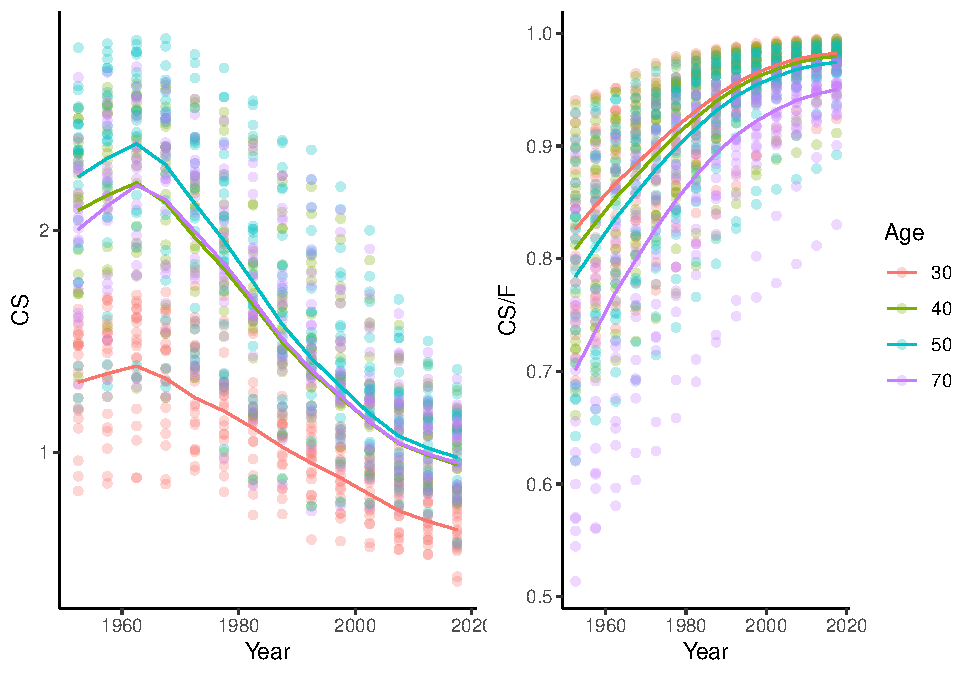
\includegraphics{paper_files/figure-latex/plot_CS-1.pdf}
\caption{Child Survival and Child survival as a share of cummulative
fertility by age, for women aged 30, 40 and 50. Estimates using UN WPP
data for Latin American countries in the period 1950-2015 period}
\end{figure}

Guatemala improved the approximation with years due to
rectangularization process in \(l_x\) (figure
@ref(fig:plot\_CS\_aprox)).

\begin{figure}
\centering
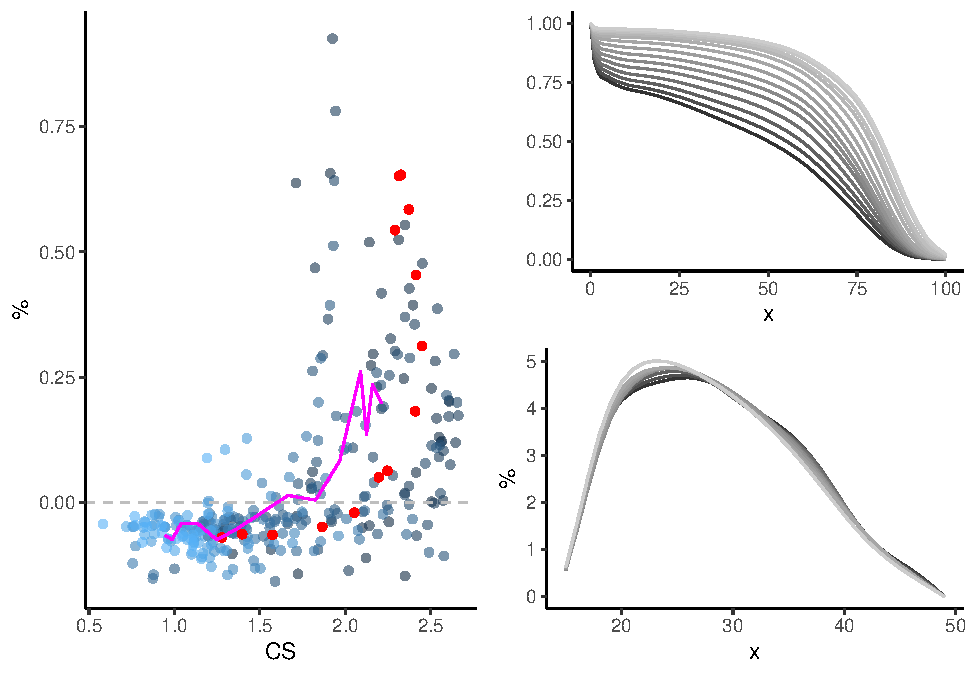
\includegraphics{paper_files/figure-latex/plot_CS_aprox-1.pdf}
\caption{Left: Error in approximation for a=40, from years 1950 (darker)
to 2015 (lighter) for all Latin American countries (blue) and Guatemala
(red). Right: Change in survival and fertility by age in Guatemala.}
\end{figure}

With \(\mu_{x+t}=\mu_x\) for \(t\) between 0 and 1,
\(\int_{x}^{x+1}{\mu_t dt} = M_x\), so discretizing
\(\frac{\Delta CS_{a}}{CS_a} \approx - \left[\sum_{0}^{a-1}{M_x \, \frac{CS_{a-1-x}}{CS_a}\,}\right] \Delta \delta\).

Assuming constant period rates the expected time in years that a mother
aged 30 passed with a death son was around 4\% in some countries at
middle XX Century. When increasing age, the survival experience depends
less on infant mortality, and the distribution is around less than 2\%
for women aged 50, converging to 0 on time. As extreme cases, in
1950-1955 Haiti women aged 30 would have experienced an intensity of
0.5\%, and in 2010-2015 0.5\%, while the women of Costa Rica 0.5\%, and
in 2010-2015 0.5\%. For those Latin American mothers aged 50 with 3
daughters born who suffered a lost, they experienced that at age 30 in
average (figure @ref(fig:plot\_ITL\_MAL)) (More can be analyzed here).

\begin{figure}
\centering
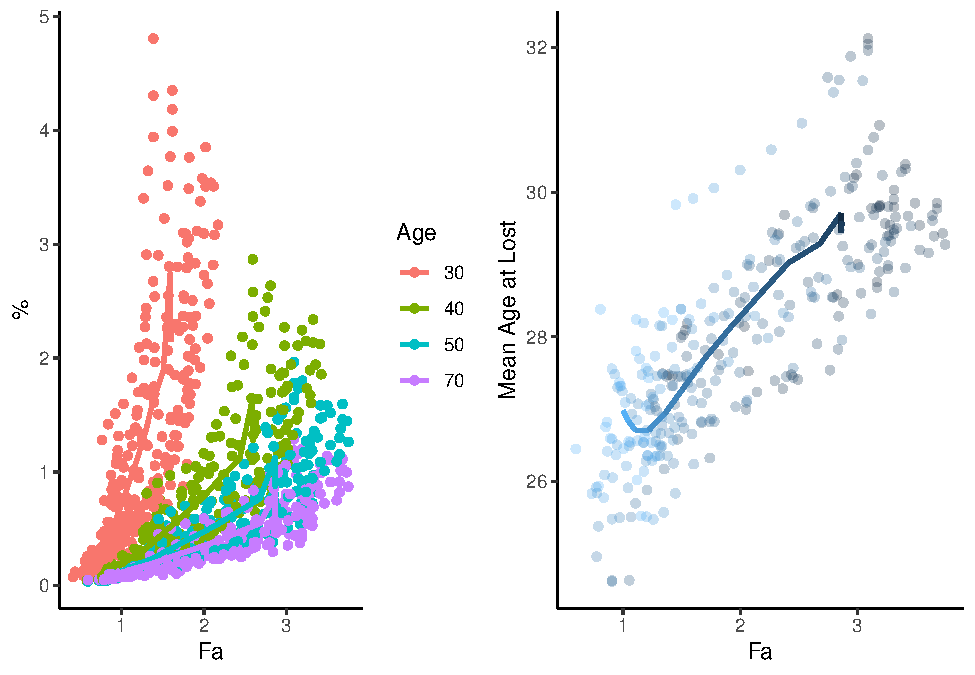
\includegraphics{paper_files/figure-latex/plot_ITL_MAL-1.pdf}
\caption{Intensity Tome Lost of womans aged 30, 40 and 50. Years 1950
(darker) to 2015 (lighter). Latinamerican countries in period 1950-2015}
\end{figure}

\hypertarget{references}{%
\subsection*{References}\label{references}}
\addcontentsline{toc}{subsection}{References}

\hypertarget{refs}{}
\begin{cslreferences}
\leavevmode\hypertarget{ref-alburez_gutierrez_womens_2019}{}%
Alburez-Gutierrez, Diego, Martin Kolk, and Emilio Zagheni. 2019.
``Women's Experience of Child Death over the Life Course: A Global
Demographic Perspective.'' Preprint. SocArXiv.
\url{https://doi.org/10.31235/osf.io/s69fz}.

\leavevmode\hypertarget{ref-bongaarts_projection_1987}{}%
Bongaarts, John. 1987. ``The Projection of Family Composition over the
Life Course with Family Status Life Tables.'' In \emph{Family
Demography: Methods and Their Application}, edited by John Bongaarts and
Thomas Burch. Oxford: IUSSP Series, Oxford Univer- sity Pres.

\leavevmode\hypertarget{ref-brass_derivation_1953}{}%
Brass, W. 1953. ``The Derivation of Fertility and Reproduction Rates
from Restricted Data on Reproductive Histories.'' \emph{Population
Studies} 7 (2): 137. \url{https://doi.org/10.2307/2172029}.

\leavevmode\hypertarget{ref-Coresh1988}{}%
Coresh, Josef, and Noreen Goldman. 1988. ``The effect of variability in
the fertility schedule on numbers of kin.'' \emph{Math. Popul. Stud.} 1
(2): 137--56. \url{https://doi.org/10.1080/08898488809525268}.

\leavevmode\hypertarget{ref-daatland_norwegian_2010}{}%
Daatland, Svein Olav, Marijke Veenstra, and Ivar A. Lima. 2010.
``Norwegian Sandwiches: On the Prevalence and Consequences of Family and
Work Role Squeezes over the Life Course.'' \emph{European Journal of
Ageing} 7 (4): 271--81. \url{https://doi.org/10.1007/s10433-010-0163-3}.

\leavevmode\hypertarget{ref-goodman1974}{}%
Goodman, Leo A, Nathan Keyfitz, and Thomas W Pullum. 1974. ``Family
Formation and the Frequency of Various Kinship Relationships.''
\emph{Theoretical Population Biology} 5 (1): 1--27.

\leavevmode\hypertarget{ref-Hendrickson2009}{}%
Hendrickson, K. C. 2009. ``Morbidity, Mortality, and Parental Grief: A
Review of the Literature on the Relationship Between the Death of a
Child and the Subsequent Health of Parents.'' \emph{Palliat Support
Care} 7 (1): 109--19.

\leavevmode\hypertarget{ref-KeyfitzMath}{}%
Keyfitz, Nathan, and Hal Caswell. 2005. \emph{Applied Mathematical
Demography}. Vol. 47. Springer.

\leavevmode\hypertarget{ref-lee_death_2014}{}%
Lee, Chioun, Dana A. Glei, Maxine Weinstein, and Noreen Goldman. 2014.
``Death of a Child and Parental Wellbeing in Old Age: Evidence from
Taiwan.'' \emph{Social Science \& Medicine} 101 (January): 166--73.
\url{https://doi.org/10.1016/j.socscimed.2013.08.007}.

\leavevmode\hypertarget{ref-livi_bacci_concise_1997}{}%
Livi Bacci, Massimo. 1997. \emph{A Concise History of World Population}.
2nd ed. Cambridge, MA: Blackwell.

\leavevmode\hypertarget{ref-lotka1931orphanhood}{}%
Lotka, Alfred J. 1931. ``Orphanhood in Relation to Demographic
Factors.'' \emph{Metron} 9 (2): 37--109.

\leavevmode\hypertarget{ref-Michalski2018}{}%
Michalski, Grigoriev, Anatoli I, and Vasily P and Gorlishchev. 2018. ``R
Programs for Splitting Abridged Fertility Data into a Fine Grid of Ages
Using the Quadratic Optimization Method.'' Max Planck Institute for
Demographic Research, Rostock, Germany.

\leavevmode\hypertarget{ref-WPP19}{}%
Nations, United. 2019. \emph{World Population Prospects 2019: Data
Booklet}.
\url{https://doi.org/https://doi.org/https://doi.org/10.18356/3e9d869f-en}.

\leavevmode\hypertarget{ref-preston1978effects}{}%
Preston, Samuel H, and others. 1978. \emph{The Effects of Infant and
Child Mortality on Fertility.} Academic Press, Inc., 111 Fifth Avenue,
New York/New York 10003, USA.

\leavevmode\hypertarget{ref-smith-greenaway_maternal_2020}{}%
Smith-Greenaway, Emily, and Jenny Trinitapoli. 2020. ``Maternal
Cumulative Prevalence Measures of Child Mortality Show Heavy Burden in
Sub-Saharan Africa.'' \emph{Proceedings of the National Academy of
Sciences}, February, 201907343.
\url{https://doi.org/10.1073/pnas.1907343117}.

\leavevmode\hypertarget{ref-Vaupel2014}{}%
Vaupel, James W., and Trifon I. Missov. 2014. ``Unobserved population
heterogeneity: A review of formal relationships.'' \emph{Demographic
Research} 31 (September): 659--86.
\url{https://www.demographic-research.org/Volumes/Vol31/22}.

\leavevmode\hypertarget{ref-Vaupel1986}{}%
Vaupel, J. W. 1986. ``How Change in Age-Specific Mortality Affects Life
Expectancy.'' \emph{Population Studies} 40 (1): 147--57.
\url{https://doi.org/10.2307/2174285}.

\leavevmode\hypertarget{ref-volk_infant_2013}{}%
Volk, Anthony A., and Jeremy A. Atkinson. 2013. ``Infant and Child Death
in the Human Environment of Evolutionary Adaptation.'' \emph{Evolution
and Human Behavior} 34 (3): 182--92.
\url{https://doi.org/10.1016/j.evolhumbehav.2012.11.007}.

\leavevmode\hypertarget{ref-wrycza2012}{}%
Wrycza, Tomasz, and Annette Baudisch. 2012. ``How Life Expectancy Varies
with Perturbations in Age-Specific Mortality.'' \emph{Demographic
Research} 27: 365--76.
\end{cslreferences}

\end{document}
